\documentclass{article}

\usepackage{graphicx}
\usepackage{amsmath}
\usepackage{hyperref}
\usepackage[utf8]{inputenc}
\usepackage{cite}
\graphicspath{ {./images/} }

\begin{document}

\title{Advancements in Healthcare by using IoT and Cloud based systems}
\author{Summary By : Vishwa Kumaresh}
\date{January 2023}

\maketitle
\tableofcontents

\begin{abstract}
The paper "Smart Healthcare System Based on Cloud-Internet of Things and Deep Learning" by Benzhen Guo, Yanli Ma, and Jingjing Yang presents a novel approach for improving healthcare delivery using advanced technologies such as cloud computing, IoT and deep learning. The authors effectively demonstrate how these technologies can be integrated to create a system that allows for real-time monitoring and analysis of patient data, as well as remote diagnosis and treatment.

One of the strengths of the paper is the clear and detailed explanation of the proposed system and its potential benefits. The authors provide a clear overview of the system's architecture and explain how the different components (such as IoT devices, cloud computing, and deep learning algorithms) work together to achieve the system's goals. They also present a thorough discussion of the potential benefits of the system, such as improved efficiency and cost-effectiveness in healthcare delivery and more personalized and effective care for patients.

However, the paper could have discussed more about the potential challenges and limitations of the proposed system. While the authors briefly mention that there may be challenges related to data privacy and security, they do not provide a detailed discussion of these issues or how they plan to address them.

Overall, the paper is well-written and provides a clear and compelling argument for the potential of using advanced technologies to improve healthcare delivery.
\end{abstract}

\section{Introduction}
The main aim of the paper is to provide a solution for remote health diagnosis and health monitoring. The authors of the paper propose the use of sensors embedded in the devices we use in our day to day lives, such as smart phones and smart bracelets, to provide timely aid to the patients and monitor them in case of any emergency. They have addressed various issues that may be faced, such as the inability to collect data from different devices, Limited memory capacity and computing power. 

The system they proposed uses a combination of Deep Learning model and Cloud-Internet of Things (C-IoT) for various steps of the system, ranging from data acquisition and data preprocessing to Evaluation and Model training 

\section{Methodology}
The authors propose a 3 layer architecture : 
\begin{enumerate}
    \item \texttt{Data Collection layer} : This layer uses the data measures from various devices like Pedometer, temperature etc. This layer detects, filters and collects the data
    \item \texttt{Data Preprocessing and Net Layer} : The data collected from the data collection layer is sent to different devices such as routers, smartphones etc. From here, the data is normalized and transformed. We also generate the Health Image from this data
    \item \texttt{Data Processing and Application Layer} : The data that is sent to the cloud will be processed using some deep learning models and new functions are generated from here
\end{enumerate}

\begin{figure}
    \centering
    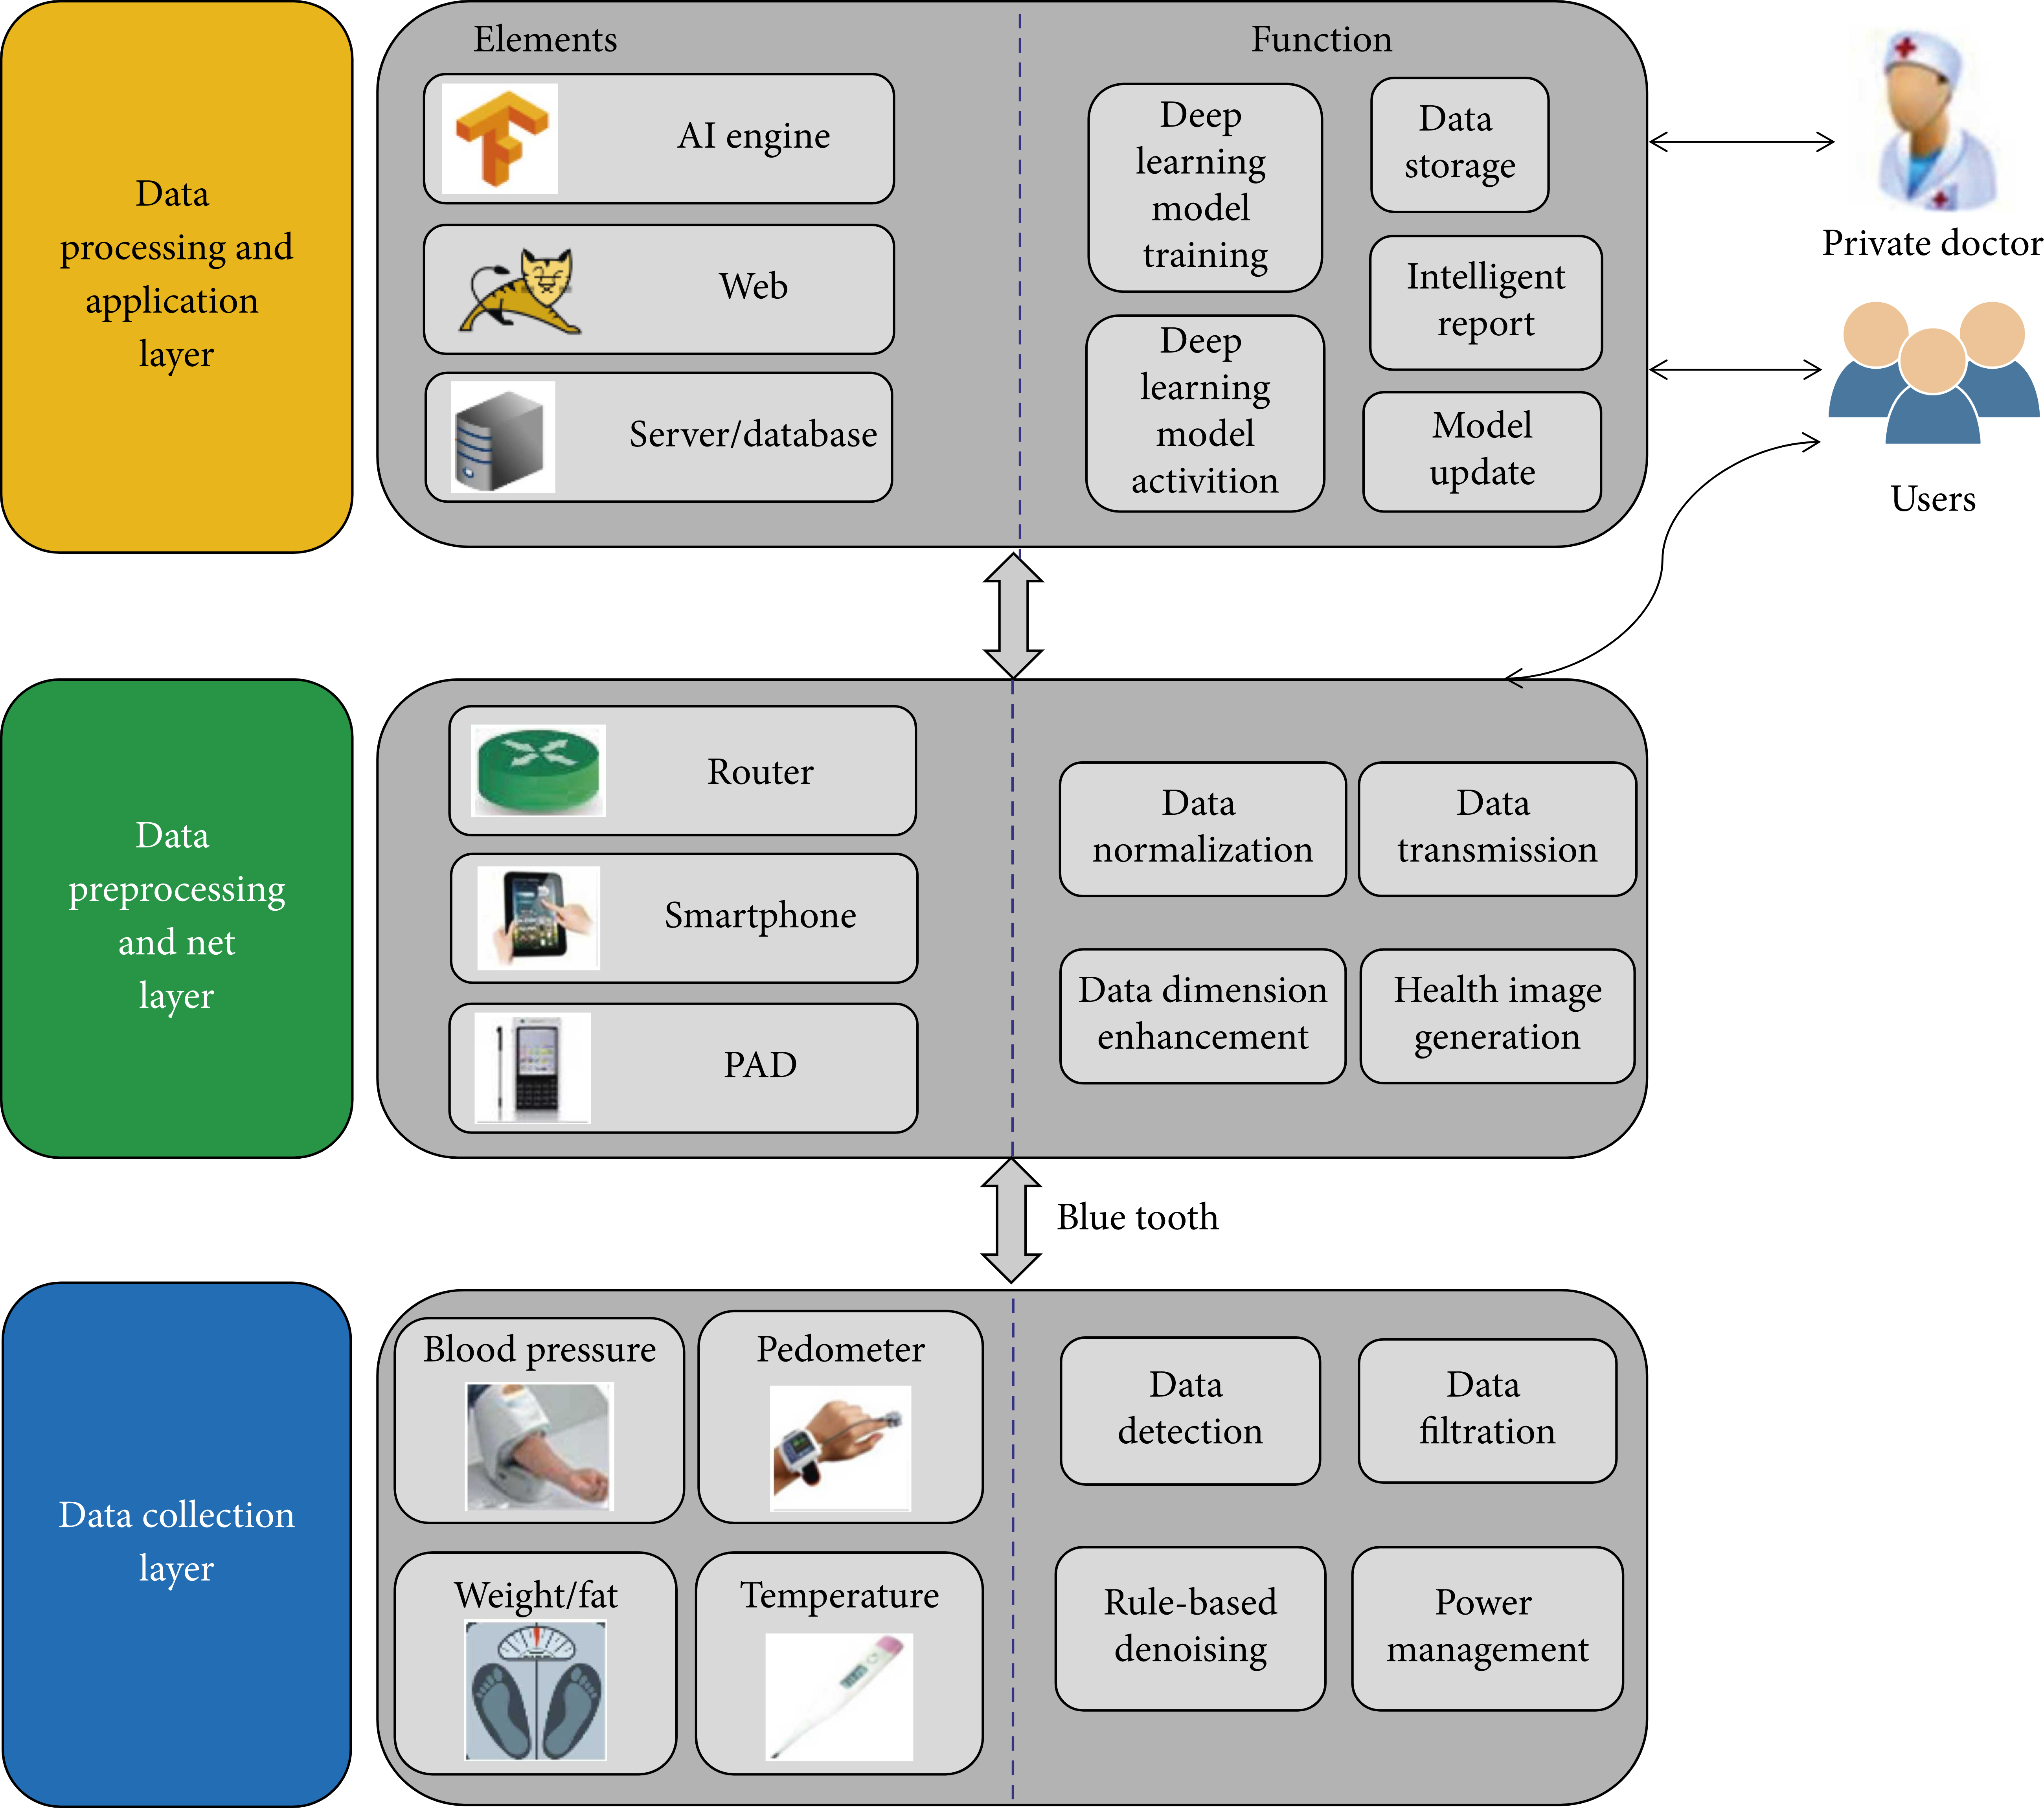
\includegraphics[width=\linewidth]{4109102.fig.001.png}
    \caption{Steps}
    \label{fig:label1}
\end{figure}


\subsection{System Architecture}
The data collection layer help to acquire the physiological parameters of health such as temperature, body fat etc. from various wearable devices. These devices have small storage and low computing capacity. High frequency noise is also eliminated here, and some special values can be eliminated based on some pre-written rules. 

The data preprocessing and net layer for medical IoT gateways are mainly composed of smartphones and other mobile devices. These devices serve as network layer devices to enable data communication and also install application layer software for local data preprocessing, device control, and parameter display. Smartphones connect to data collection devices through Bluetooth to receive measurement information and display it on mobile apps. Preprocessed data is then uploaded to cloud servers through various communication methods. Data preprocessing includes normalization, dimension transformation, and data fusion to generate images of health parameters.

We need to ensure that the server is well secured as we are dealing with the private data of various people. We also update the model based on the data provided by the doctor. 

\subsection{Measurement of Blood Pressure}
It can be calculated using the equation :

\begin{equation}
    B = (X^T X)^-1 X^T Z
\end{equation}
The estimated parameters \begin{equation} (b_0, b_1, b_2) \end{equation} are substituted into equation (1) to obtain the fitted Gaussian function. 

\subsection{Data Preprocessing}
The data preprocessing is done on the mobile device after the data is transmitted. The main outcomes of this stage is dimensional transformation of data, data standardization, and generation of two-dimensional gray image for human health. 

(Here, the acronyms are mean arterial pressure (MAP), ambulatory pulse pressure (APP), and ambulatory rate-pressure product (ARPP))

Functions used :
\begin{equation}
    APP = F1(SP, DP) = SP - DP
\end{equation}
\begin{equation}
    MAP = F2(SP, DP) = \frac{DP + (SP - DP)}{3}
\end{equation}
\begin{equation}
    ARPP = F3(HR, SP) = HR * SP
\end{equation}

Image of Human Health : 
\begin{figure}
    \centering
    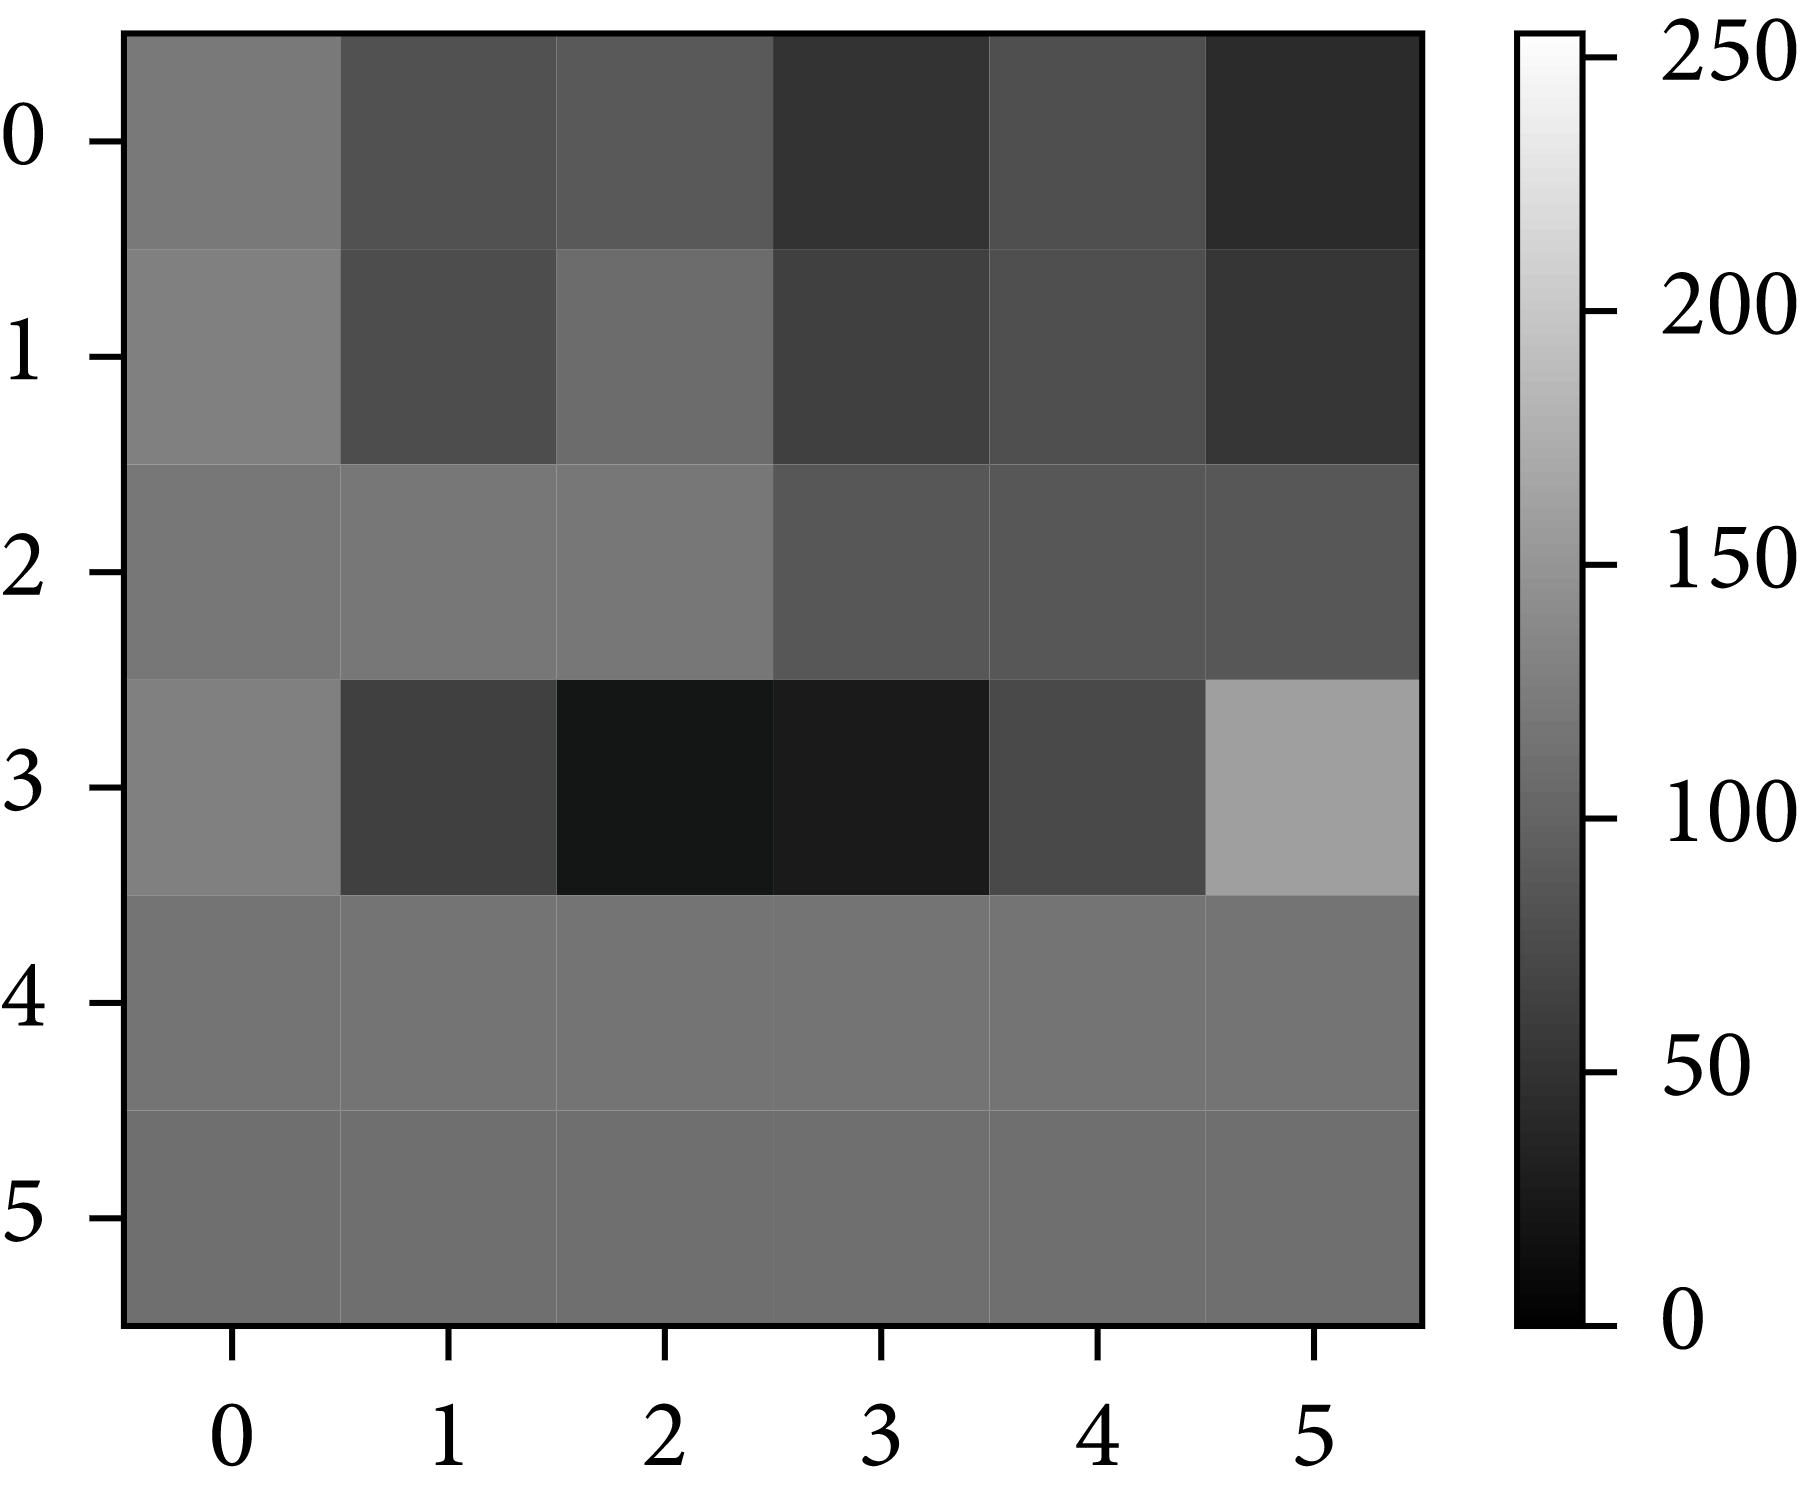
\includegraphics[width=\linewidth]{4109102.fig.003.png}
    \caption{Human Health Map}
    \label{fig:label2}
\end{figure}


\subsection{Collection of Data}
The data collection of this experiment was done with 6 people, including 3 males and 3 females (including 2 adolescents, 2 middle-aged, and 2 elderly)

\subsection{Deep Learning Model}
The Model used is a simple CNN model. They have used the LeNet-5 CNN model and adopted and modified it to simplify a pooling layer.


\section{Results and Discussion}
\subsection{Measurement and Test of blood pressure}
They have compare the methods of using blood pressure meter and blood pressure measurement node at the same time for the same subject. They had found out that the error was withing 6\%.

\subsection{Evaluation of Deep Learning Algorithm and Model}
Precision, Recall and F1 scores were used to evaluate the model

\section{My Thoughts and Views}
I believe that in this paper, although a better system than the current status quo was proposed, it is not without its flaws. For this system to work, it need a large about of data for training. Also, the model constantly needs to be updated based on the inputs from doctors. For this system to work, the patients need to be constantly connected to their wearable devices and must also allow information to be sent to the cloud. Also, the tests were not done on a sufficiently large sample size so as to draw any meaningful conclusions.

A better system than this can be easily implemented by using better IoT sensors that can take in data in a more precise way, such as accurate calculation of blood pressures.

\section{Conclusion}
Although the proposed system has a few drawbacks, implementing it and using it will still be quite helpful as it will allow doctors to remotely monitor the patient and provide a timely treatment in case of any emergency for the patient.


\section*{Submission Details}
\begin{itemize}
    \item Name : Vishwa Kumaresh
    \item Roll number : 21011101055
    \item Reg number : 21110226
    \item Class : AI and DS, Section A
    \item \href{https://www.hindawi.com/journals/jhe/2021/4109102/}{Link to Paper}
\end{itemize}

\end{document}
\bibliography{citation.bib}

%\ref
%\label